\documentclass{eecslides}
\usepackage{amsmath}

%------------------------------

\title[Network biogeography]{A quantitative framework for network biogeography}
\author[D. Gravel]{Dominique Gravel}
\institute{UQAR -- Canada Research Chair in Ecosystem ecology}
\website{http://www.chaire-eec.uqar.ca/}
\date{\today}

\begin{document}

	\begin{frame}[plain]
		\titlepage
	\end{frame}

%------------------------------

	\section{Introduction}

%------------------------------

	\begin{frame}{Biogeography of ecological interactions}{Challenge of getting network data at large spatial scales}
 	    	\begin{columns}
			\begin{column}{0.4\textwidth}			
				\begin{itemize}
					\item Hard to document;
					\item Usually not replicated;
					\item Applies only to co-occurring species;
					\item Network structure is deterministic and stationary.
				\end{itemize}
			\end{column}
%----
			\begin{column}{0.6\textwidth}
				\begin{center}
					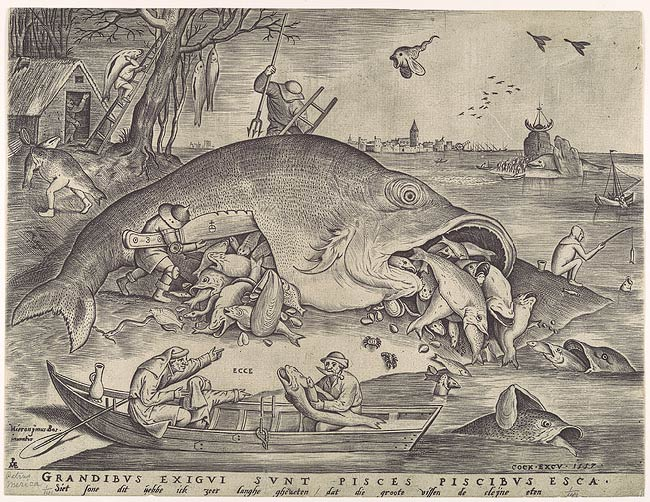
\includegraphics[height=0.55\textheight]{bruegel}\\
				\end{center}
			\end{column}				
		\end{columns}	   
	\end{frame}

%------------------------------

	\begin{frame}{Biogeography of ecological interactions}
		\begin{center}
			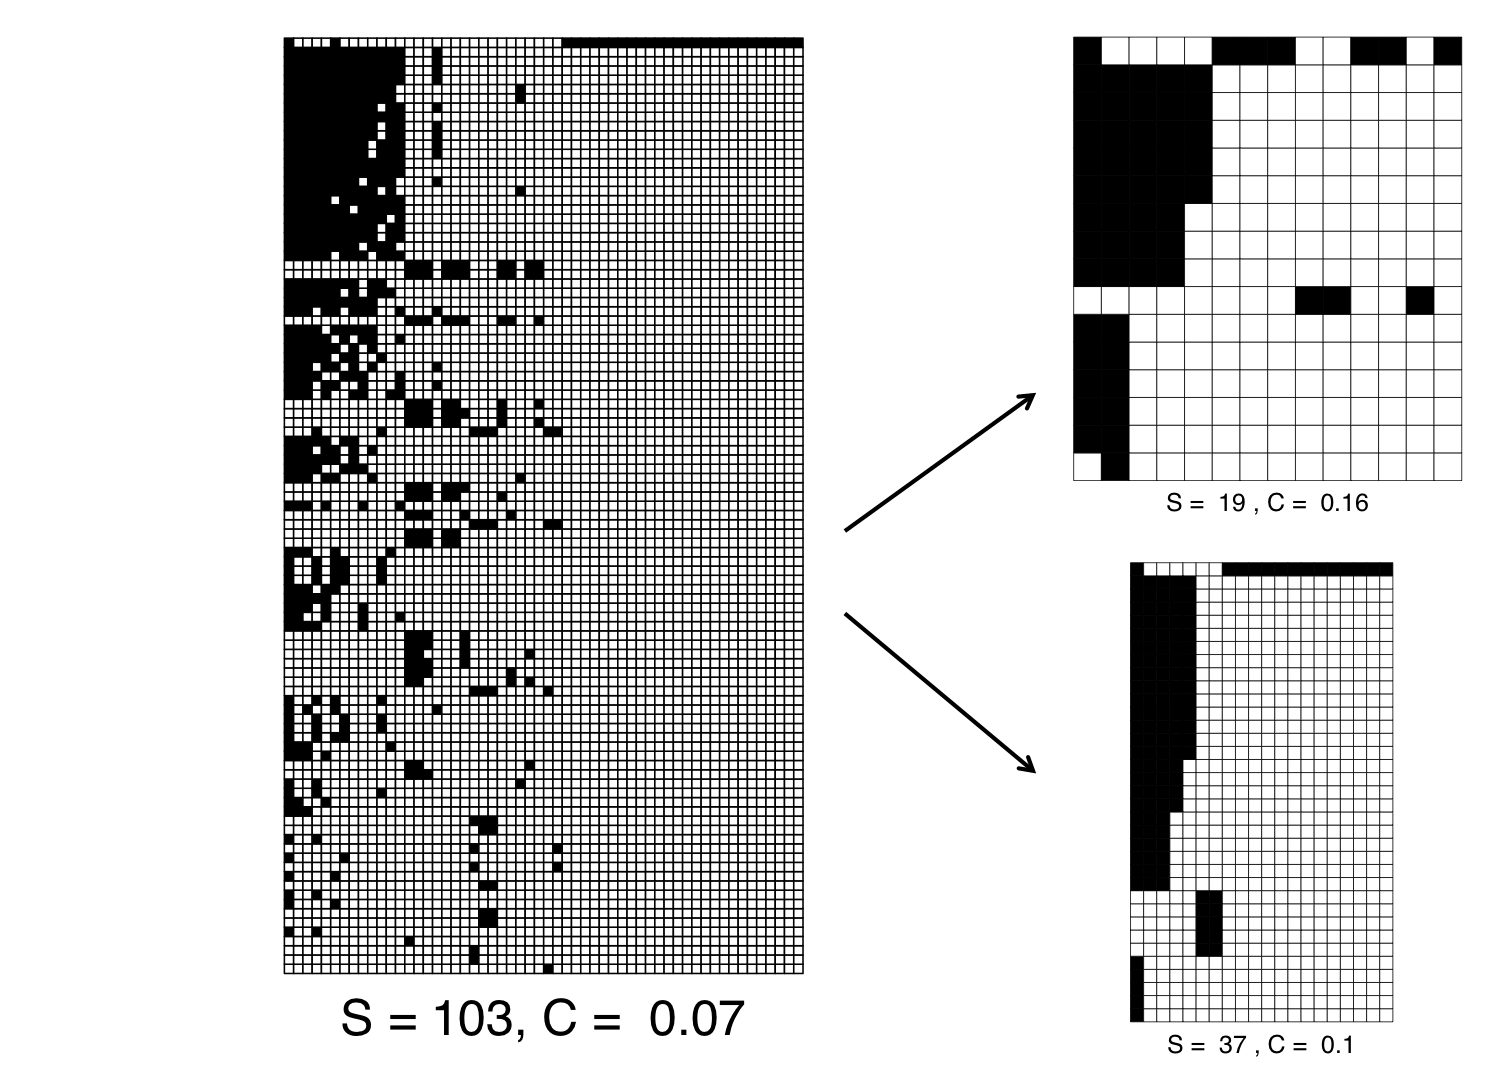
\includegraphics[height=0.55\textheight]{havens_sampling}\\
			\footnotesize{Gravel et al. (2011). \textit{Ecol. Lett.}}
		\end{center}   
		\begin{center}
			\alert{\textbf{How can we predict do local networks assemble from the metaweb?}}
		\end{center}	 	    
	\end{frame}

%------------------------------

	\begin{frame}{Biogeography of ecological interactions}
		\begin{center}
			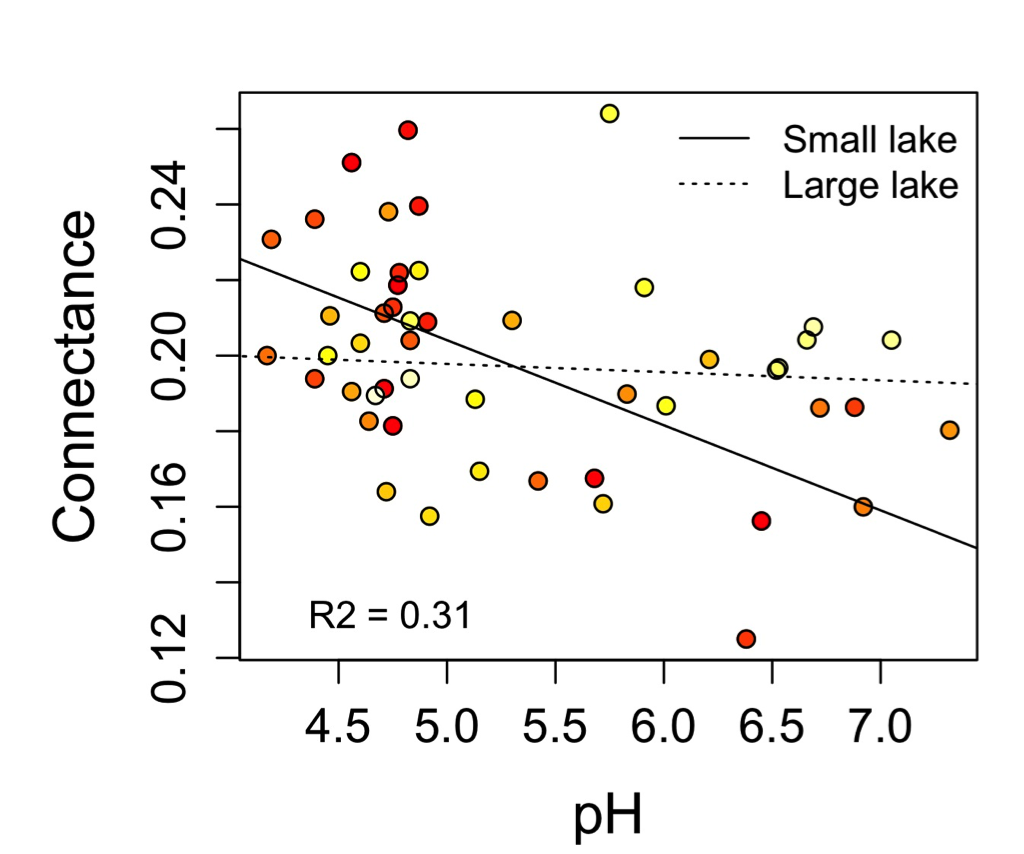
\includegraphics[height=0.6\textheight]{havens_ph}\\
			\footnotesize{Gravel et al. (2011). \textit{Ecol. Lett.}}
		\end{center}   
	\end{frame}

%------------------------------

	\begin{frame}{Spatial variation of interaction networks}
		\begin{center}
			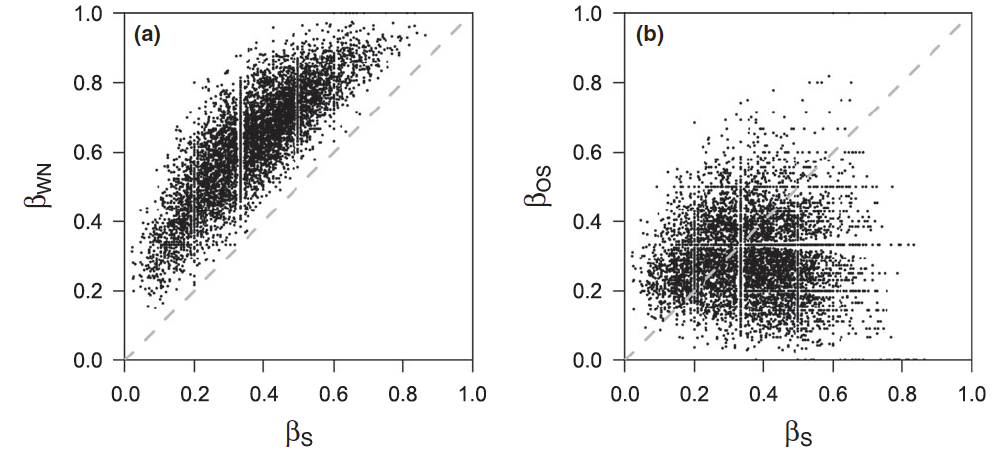
\includegraphics[height=0.45\textheight]{poisot2012}\\
			\footnotesize{Poisot et al. (2012). \textit{Ecol. Lett.}}
		\end{center} 

		Networks do vary in space because of:
			\begin{itemize}
				\item Species turnover;
				\item Link turnover;
			\end{itemize}	    
	\end{frame}

%------------------------------

	\begin{frame}{Objective}
		\begin{center}
			\alert{\large{\textbf{Propose a quantitative framework to understand and predict the spatial variation in network structure at the biogeographical scale}}}
		\end{center}	  	    
	\end{frame}

%------------------------------

	\section{Framework}

%------------------------------

	\begin{frame}{Framework}{Formulating network sampling as a stochastic process}

	Define the stochastic variable $X_{iz}$ representing the occurrence of species $i$ at the location $z$. \\
	\vskip 1em

	And the variable $L_{ijz}$ representing the occurrence of an interaction between species $i$ and $j$ at location $z$.	
	\vskip 1em

	We are looking for the probability that an interaction occurs given the environment $E_z$:
		\begin{center}
			$P(L_{ijz} = 1,X_{iz} = 1,X_{jz} = 1|E_z)$
		\end{center}	

	\end{frame}

%------------------------------

	\begin{frame}{Conditional probabilities}
	Obtained from the product rule we get:
		\begin{center}
			$P(L_{ijz},X_{iz},X_{jz}|E_z) = P(L_{ijx}|X_{ix},X_{jx}|E_z)P(X_{ix},X_{jx}|E_z)$
		\end{center}
	Where:\\
	$P(L_{ijz}|X_{iz},X_{jz}|E_z)$ is the metaweb\\
 	$P(X_{iz},X_{jz}|E_z)$ is the co-occurrence matrix
		
	\end{frame}

%------------------------------

	\begin{frame}{Interpretation}
 	    	\begin{columns}
			\begin{column}{0.3\textwidth}			
				$P(L_{ijx}|X_{iz},X_{jz}|E_z)$ is the Eltonian niche\\
			 	$P(X_{ix},X_{jz}|E_z)$ is the Grinnellian niche
			\end{column}
%----
			\begin{column}{0.7\textwidth}
				\begin{center}
					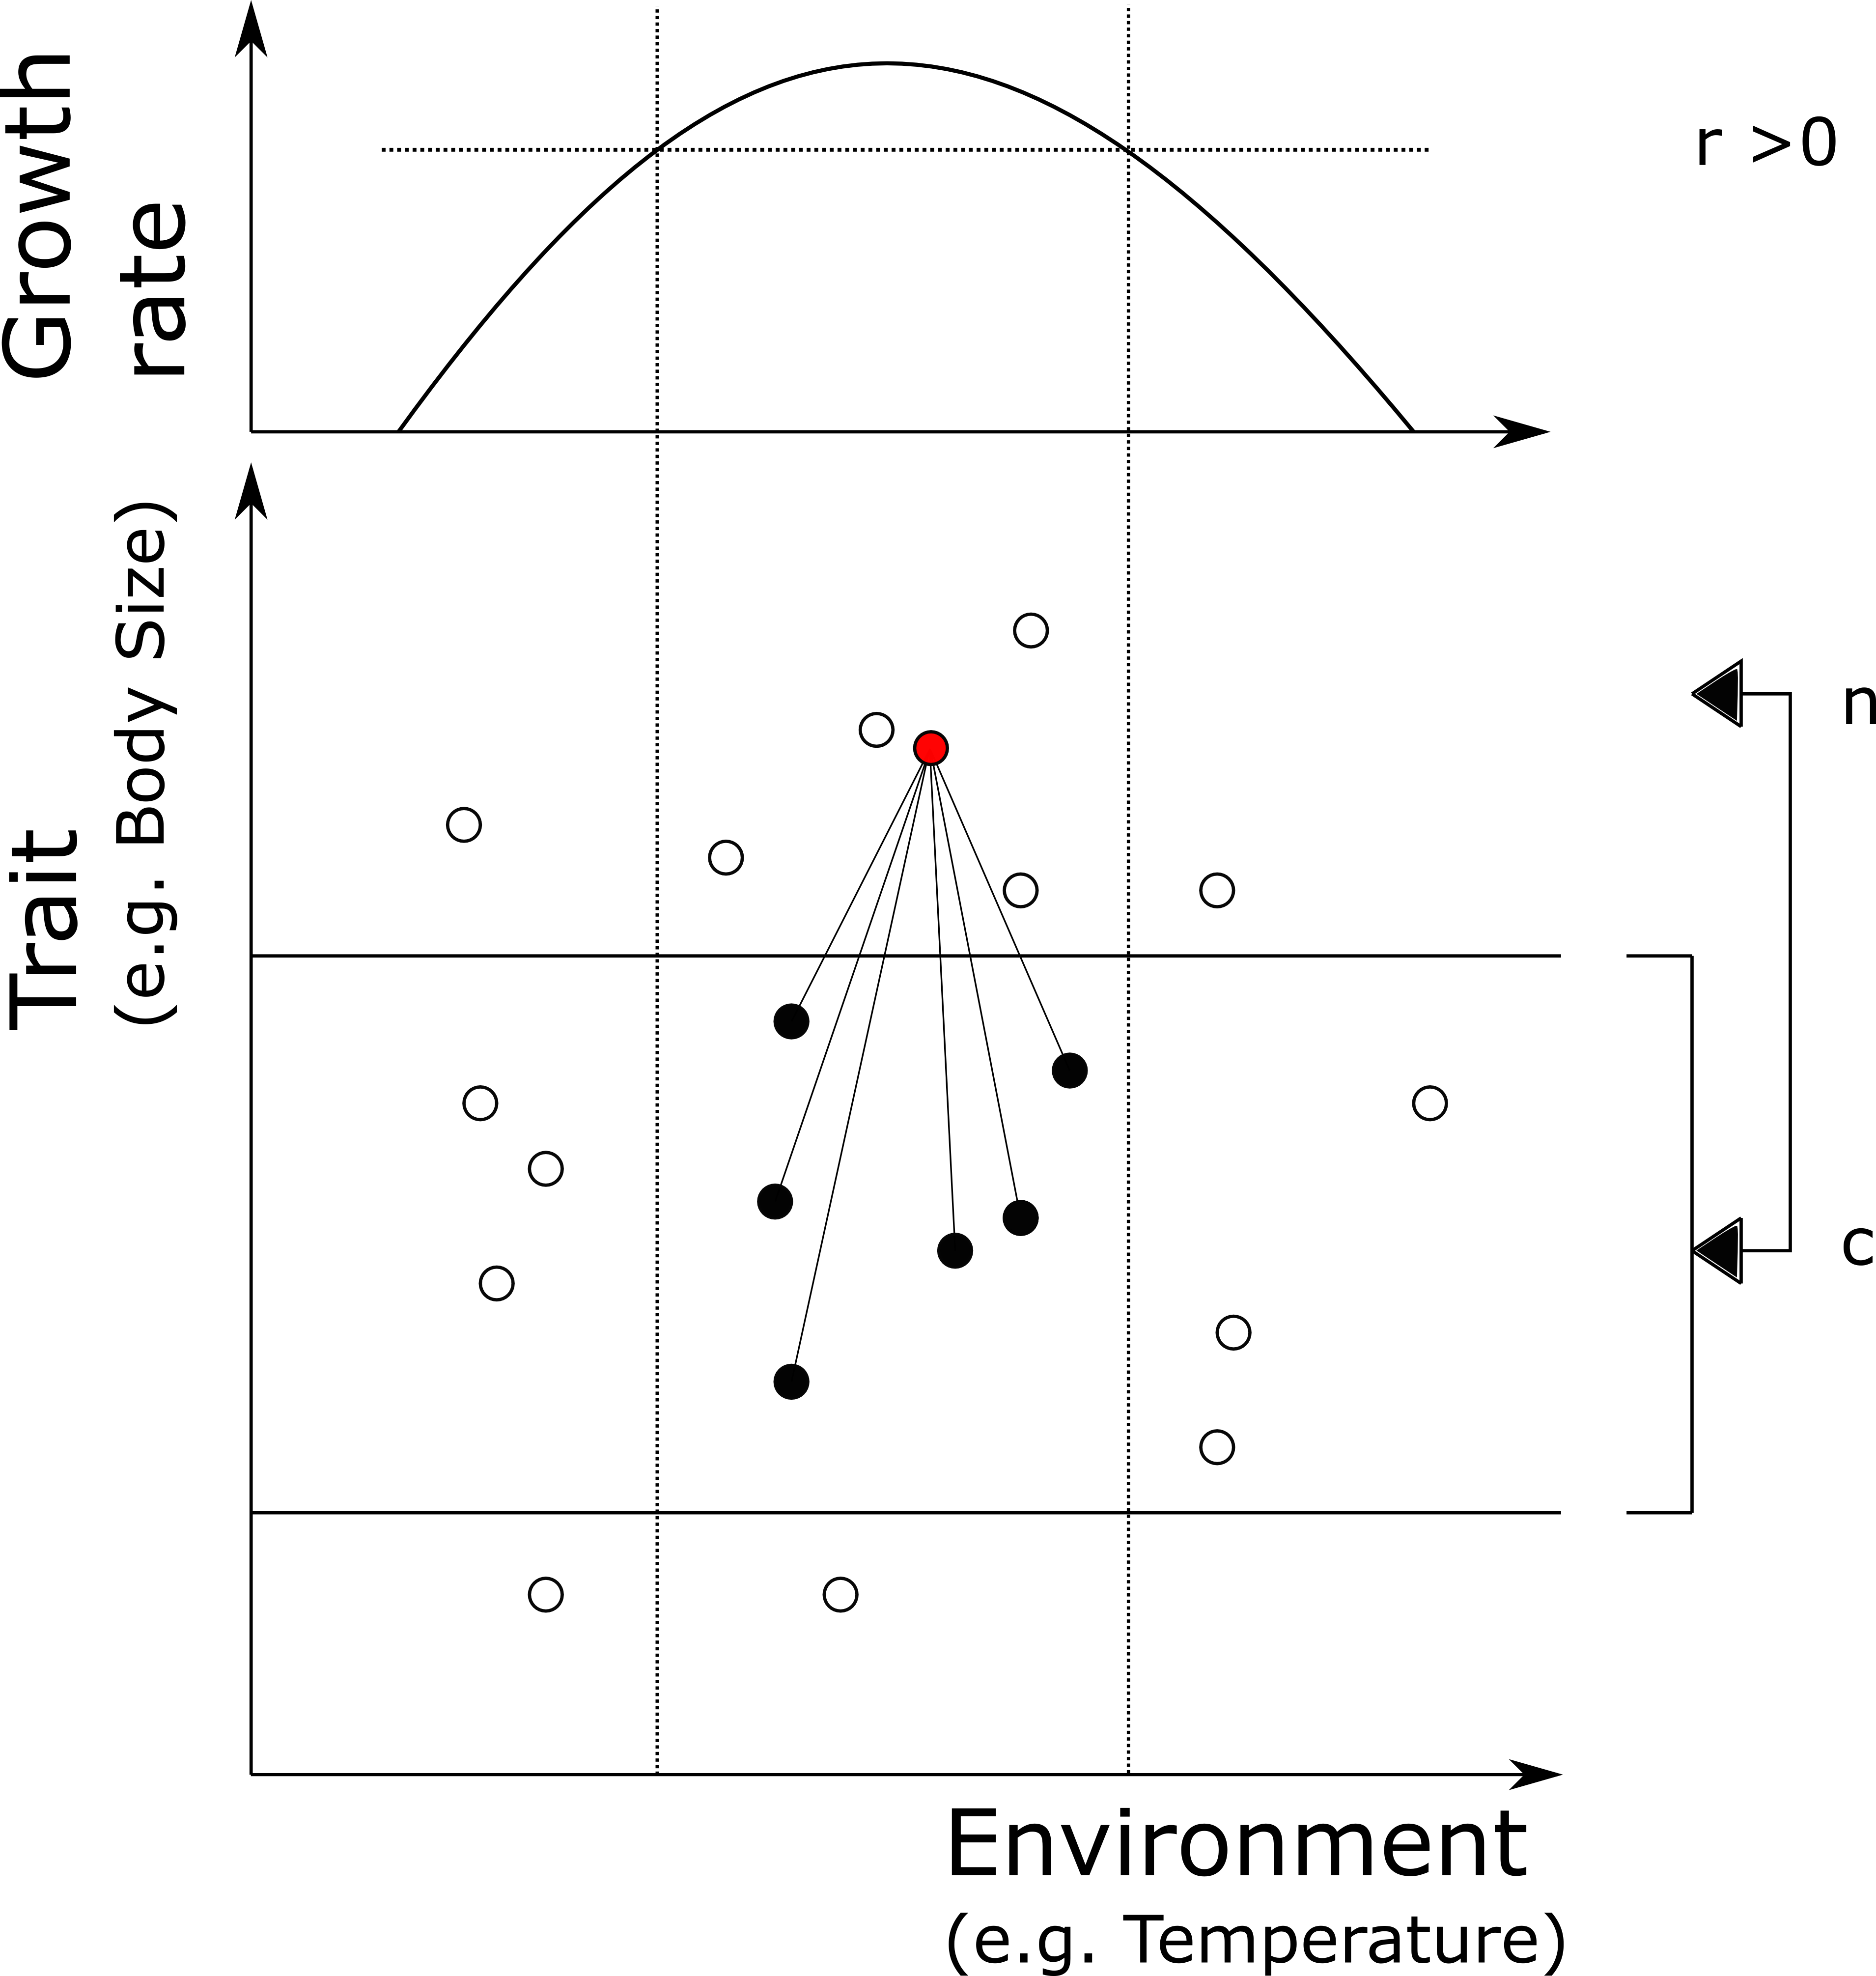
\includegraphics[height=0.65\textheight]{niche}\\
				\end{center}
			\end{column}				
		\end{columns}	   
	\end{frame}

%------------------------------

	\section{Metaweb}

%------------------------------

	\begin{frame}{Building the metaweb}
	 \alert{\textbf{The problem: inferring interactions for species that never co-occurred and with incomplete data}}
	\end{frame}

%------------------------------

	\begin{frame}{Inferring the metaweb from traits}
		\begin{center}
			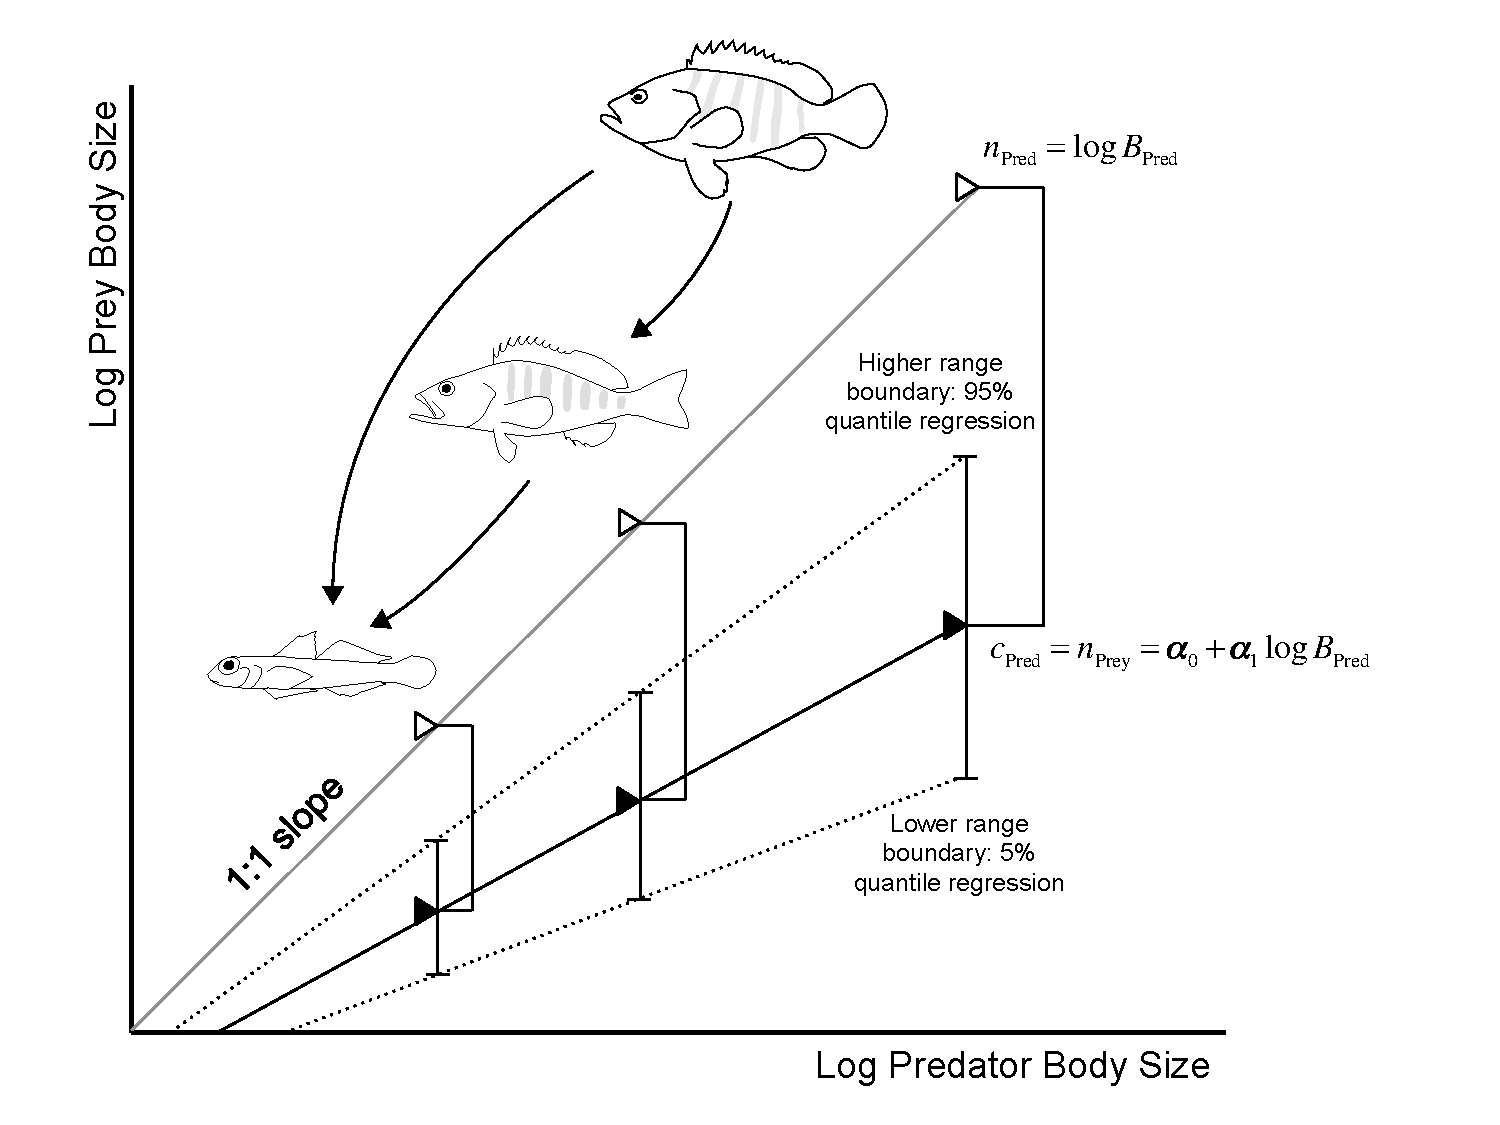
\includegraphics[height=0.55\textheight]{fig_MEE}\\
			\footnotesize{Gravel et al. (2013). \textit{Meth. Ecol. Evol.}}
		\end{center}
	\end{frame}

%------------------------------

	\begin{frame}{Bayesian formulation of the interaction probability}
 	    	\begin{columns}
			\begin{column}{0.4\textwidth}							
			The likelihood function: \\
			$P(M_{prey}|L,E_z) = \frac{P(L_{ijz}|M_{prey},M_{pred},E_z)P(M_{prey})}{P(L|M_{pred})}$
			\end{column}
%----
			\begin{column}{0.6\textwidth}
				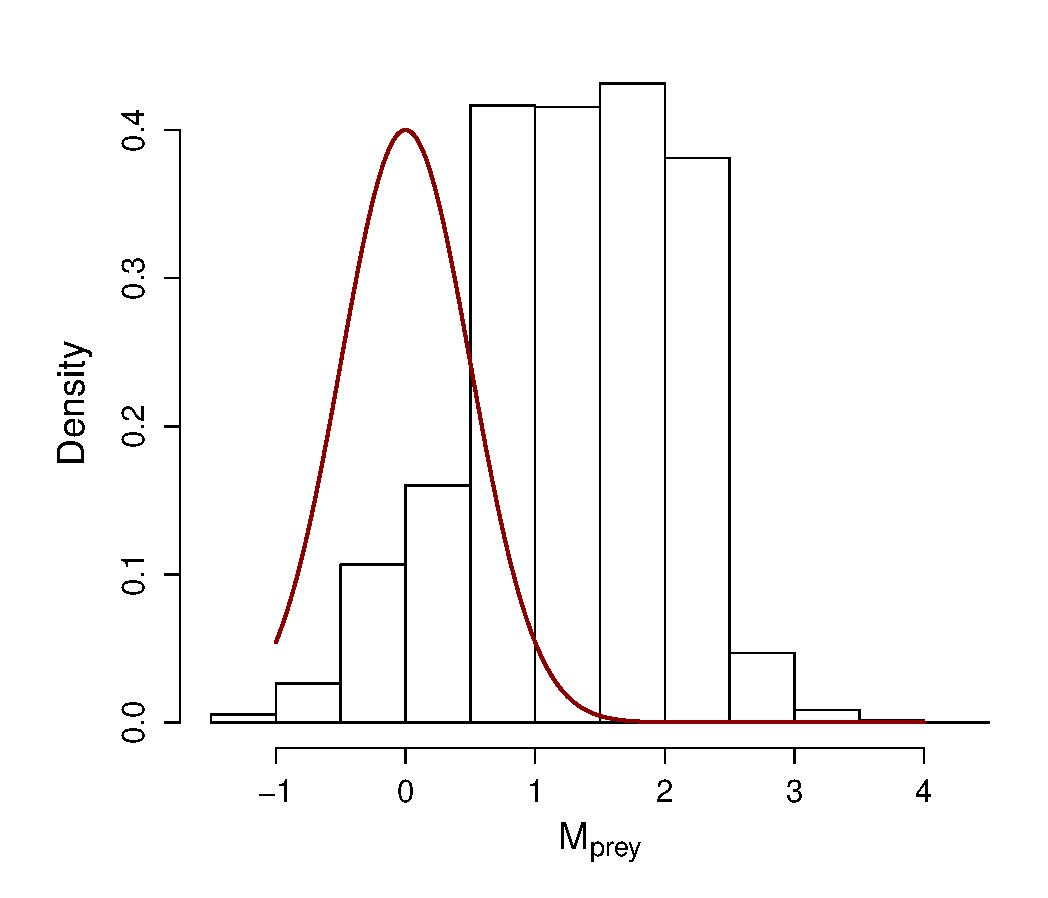
\includegraphics[height=0.6\textheight]{prey_freq}\\
			\end{column}				
		\end{columns}	   
	\end{frame}

%------------------------------

	\begin{frame}{Probalistic model}
 	    	\begin{columns}
			\begin{column}{0.4\textwidth}							
				\begin{itemize}
					\item Data from Barnes et al. (2008), Predator and prey body sizes in marine 						food webs, Ecology 86: 881;
					\item 34 931 recorded interactions;
					\item 25 sites.
				\end{itemize}
			\end{column}
%----
			\begin{column}{0.6\textwidth}
				\begin{center}
					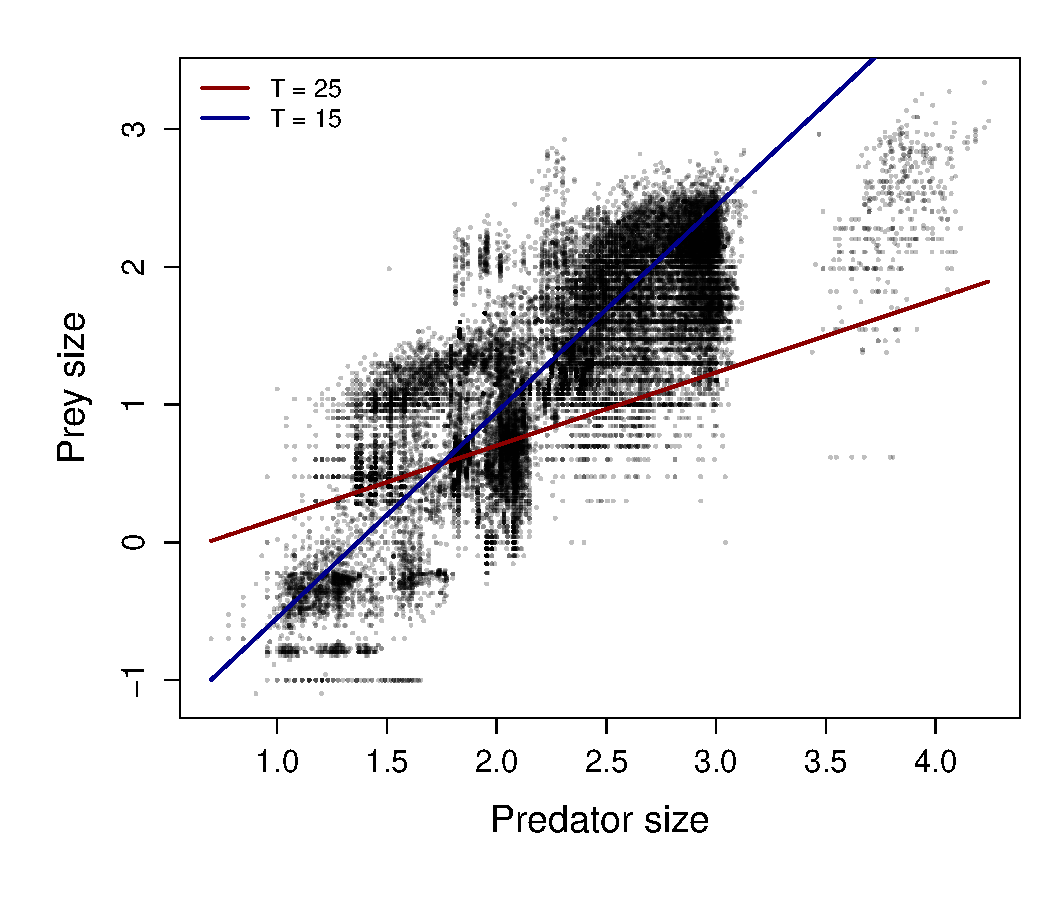
\includegraphics[height=0.6\textheight]{PredPreyTemp}\\
					\footnotesize{(see Gibert and Delong (in press) \textit{Bio. Lett.})}
				\end{center}
			\end{column}				
		\end{columns}	   
	\end{frame}

%------------------------------

	\begin{frame}{Effect of temperature on the metaweb}
		\begin{center}
				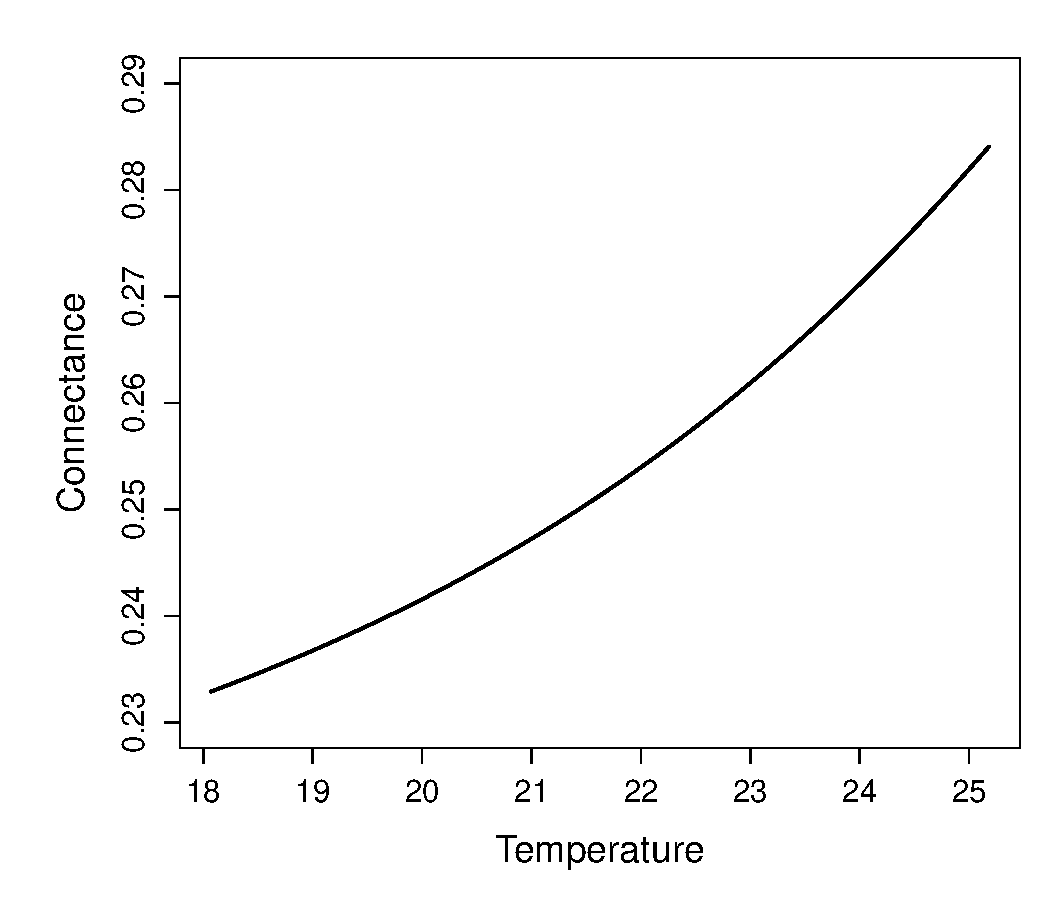
\includegraphics[height=0.65\textheight]{ConnectanceTemp}\\
		\end{center}
	\end{frame}

%------------------------------

	\section{Distribution}

%------------------------------

	\begin{frame}{Distribution}
		\begin{center}
			\alert{\textbf{How to add the effect of species distribution on the network properties?}}
		\end{center}
	\end{frame}

%------------------------------

	\begin{frame}{Distribution of Mediterranean fish networks}
 	    	\begin{columns}
			\begin{column}{0.3\textwidth}							
				Neutral species distribution: \\
				$P(X_{iz},X_{jz}|E_z) = P(X_{iz}|E_z)P(X_{jz}|E_z)$
			\end{column}
%----
			\begin{column}{0.7\textwidth}
				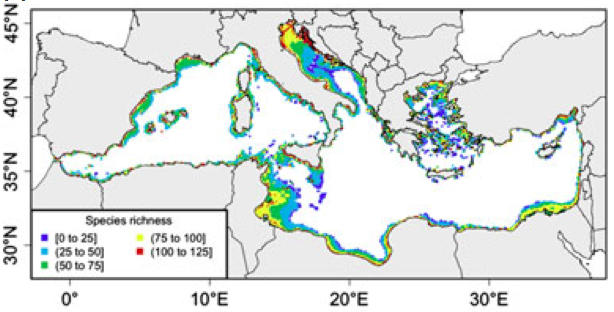
\includegraphics[height=0.4\textheight]{med_richness}\\
				\footnotesize{Albouy et al. (2014). \textit{Glob. Change Biol.}}
			\end{column}				
		\end{columns}	   
	\end{frame}

%------------------------------

	\begin{frame}{Distribution of connectance}
 	    	\begin{columns}
			\begin{column}{0.5\textwidth}							
				\begin{center}
					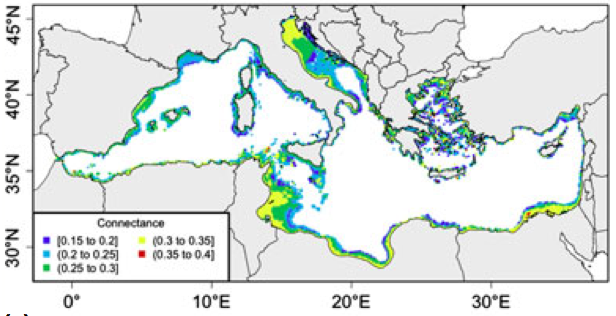
\includegraphics[height=0.3\textheight]{med_connectance}\\
					\footnotesize{Albouy et al. (2014). \textit{Glob. Change Biol.}}
				\end{center}
			\end{column}
%----
			\begin{column}{0.5\textwidth}
				\begin{center}
					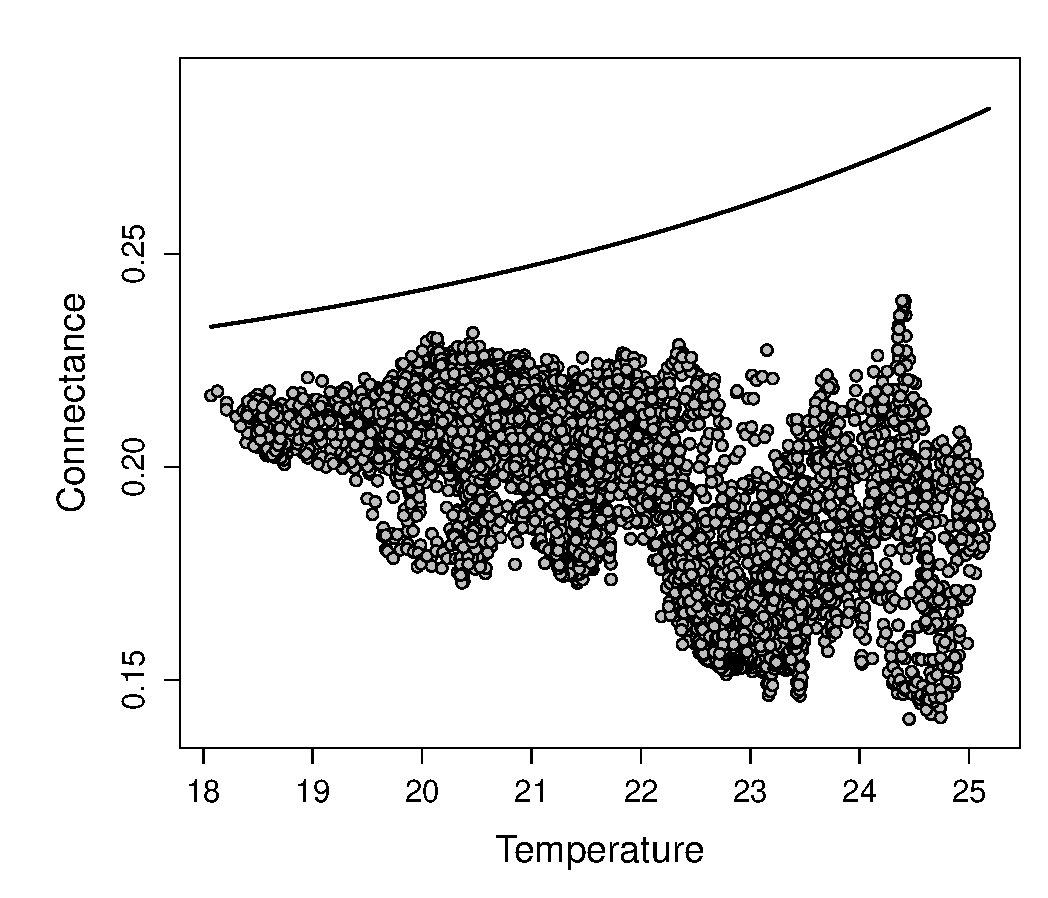
\includegraphics[height=0.5\textheight]{ConnectanceTempSDM}\\
				\end{center}
			\end{column}				
		\end{columns}	   
	\end{frame}

%------------------------------

%	\begin{frame}{Signature of temperature on the metaweb}
%		\begin{center}
%%				\includegraphics[height=0.65\textheight]{modularityTemp}\\
%		\end{center}
%	\end{frame}

%------------------------------

	\section{Discussion}

%------------------------------

	\begin{frame}{Summary}{Theory for network variation in space}
		The multiple roles of the environment on network structure: 
		\begin{itemize}
			\item Predator-prey body size relationship
			\item Regional species pool 
			\item Species distribution
		\end{itemize}
	\end{frame}

%------------------------------

	\begin{frame}{Outlook}{Dynamic modeling}

 	    	\begin{columns}
			\begin{column}{0.45\textwidth}							
				Additional sources of information: 
					\begin{itemize}
						\item Phylogeny
						\item Feedback between interactions and co-occurrence
						\item Habitat area and isolation
					\end{itemize}

			\end{column}
%----
			\begin{column}{0.55\textwidth}
				\begin{center}
					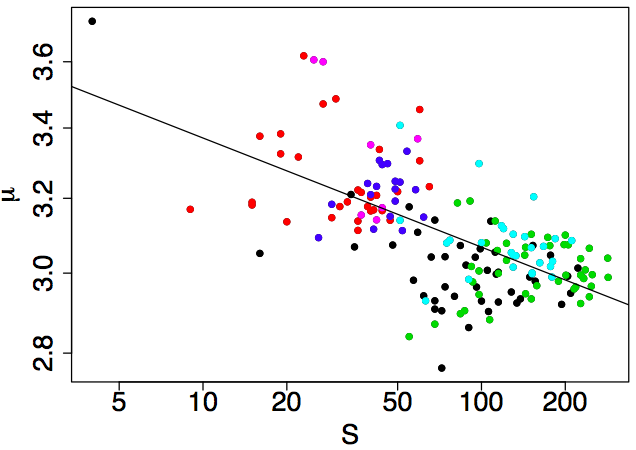
\includegraphics[height=0.45\textheight]{size_reefs}\\
				\end{center}
			\end{column}				
		\end{columns}	   
	\end{frame}

%------------------------------

	\begin{frame}{Acknowledgements}
	    
	\textbf{Co-authors:} Camille Albouy, Timothée Poisot, SFI Working group on gradient-based network research; CIEE Working group on spatial variation in network structure\\
	\vskip 1em
	\textbf{Funding:} NSERC, FRQNT, Canada Research Chair program, Quebec Center for Biodiversity Sciences, Santa Fe Institute, UQAR, CIEE.

	\end{frame}

%------------------------------

\end{document}